\documentclass[conference]{IEEEtran}
\IEEEoverridecommandlockouts
% The preceding line is only needed to identify funding in the first footnote. If that is unneeded, please comment it out.
\usepackage{cite}
\usepackage{amsmath,amssymb,amsfonts}
\usepackage{algorithmic}
\usepackage{graphicx}
\usepackage{hyperref}
\usepackage{textcomp}
\usepackage{xcolor}
\def\BibTeX{{\rm B\kern-.05em{\sc i\kern-.025em b}\kern-.08em
    T\kern-.1667em\lower.7ex\hbox{E}\kern-.125emX}}

\hypersetup{
    colorlinks=true,
    linkcolor=blue,
    filecolor=magenta,
    urlcolor=cyan,
}

\begin{document}

\title{Machine Learning Project Report}

\author{
\IEEEauthorblockN{Rodrigo Castiel}
\IEEEauthorblockA{\textit{Center for Informatics} \\
\textit{Federal University of Pernambuco}\\
Recife, Brazil \\
rcrs2@cin.ufpe.br}
}


\maketitle

\begin{abstract}
In the first part of this report, we compare $k$-means to KCM-F-GH, its hard clustering variation in feature space proposed by Carvalho et al \cite{b1}.
Both methods are evaluated on the segmentation dataset available in \cite{b2} by 
computing the adjusted rand index to analyze the similarity between the predicted cluster solutions and the ground-truth labels.
In the second part, we perform a comparative analysis between three classifiers: a maximum likelihood gaussian estimator, a $k$-nearest neighbors classifier and a hybrid-model committee classifier.
Those classifiers are also tested on the segmentation dataset.
We run cross-validation multiple times to estimate the accuracy and the error margin of each classifier.
At the end, we perform Friedman test to determine the best algorithm.
Our results show that KCM-F-GH outperforms the standard $k$-means in most cases, with the tradeoff of being considerably more time-consuming.
In the second part, our experiments show that both KNN and the hybrid classifier are equally accurate in the dataset, and better than the maximum-likelihood estimator.


\end{abstract}

\begin{IEEEkeywords}
clustering, supervised learning, classification, pattern recognition
\end{IEEEkeywords}

\section{Introduction}
This research report contains two main sections.
The first one briefly describes how $k$-means and KCM-F-GH were implemented, and how they performed in the experiments.
In the second one, we point some implementation strategies for the maximum likelihood gaussian estimator (MLE), the $k$-nearest neighbors classifier (KNN) and the hybrid-model committee classifier. Then, we compare their accuracy in a series of experiments.

The \textit{Python} code, the development history and the dataset are all available on Rodrigo Castiel's personal github (click \href{https://github.com/RodrigoCastiel/am_f}{here}).
Basic repository structure:
\begin{itemize}
\item \textit{part\_1.py}: main script for running and comparing the clustering algorithms.
\item \textit{part\_2.py}: main script for running and comparing the supervised classifiers.
\item \textit{classifiers}: contains a list of classes, each implementing a classifier or a clustering algorithm.
\item \textit{core}: contains \textit{data\_loader.py}, a utility module for managing the segmentation data.
\item \textit{data}: training and test datasets.
\end{itemize}

Additionally, we use \textit{Numpy} and \textit{Scikit}, \textit{Python} libraries for linear algebra, statistics and learning utilities.

\section{Part I - Clustering}

\subsection{Implementation}

The test code start point is located in \textit{part\_1.py}.
The script arguments, to be passed in from the terminal, are a list of views which will be tested.
For example the list \textit{RGB} and \textit{SHAPE} tells the program to run both $k$-means and KCM-F-GH on the RGB and the shape view, separately.
For each view, the script then builds each classifier and calls the method fit on it.
The parameter $num\_times$ controls how many times KCM-F-GH will be executed before the best fit run is taken.
The implementation of $k$-means and KCM-F-GH are located in \textit{k\_means\_clustering.py} and \textit{kcm\_f\_gh\_clustering.py}, respectively.
They are both thoroughly documented.

\textbf{Note}. During the initial tests of KCM-F-GH, we noticed that the update of the hyper-width parameters is not robust to constant-valued features.
That is, if at a given moment a specific feature becomes constant within each cluster, the denominator of equation (24) becomes $0$ \cite{b1}, which breaks the execution.
It means that before actually running this algorithm in feature space, we must remove redudant dimensions in the dataset.
For this reason, we removed the features "REGION-PIXEL-COUNT" and "SHORT-LINE-DENSITY-2" from the shape view.

\subsection{Experiments and Results}

In the first experiments, we noticed that KCM-F-GH takes an average of approximately one hour to converge on the test dataset containing $2100$ points.
Since our personal computer's hardware is not powerful, executing KCM-F-GH $100$ times per view is impossible in practice.
Instead, we run it only $50$ times on the combined views, $10$ times on the separate views.

Figure \ref{part_i_full} shows the output log of Part I on the full view (RGB + shape views).
In this case, KCM-F-GH achieves $adjusted\_rand\_index = 0.4906$, outperforming $k$-means with $adjusted\_rand\_index = 0.2826$.
However, each run of $k$-means converges in less than a minute, whereas KCM-F-GH takes nearly one hour to converge.

In Figure \ref{part_i_rgb}, we can see that $k$-means performs better on the pure RGB view with $adjusted\_rand\_index = 0.3990$, while KCM-F-GH's accuracy drops to $0.4692$.
Notice that KCM-F-GH converges in less than $15$ iterations on the RGB in all runs.
On the full view, it may take up to $30$ iterations, but in the average it converges in $15$ iterations.

The shape view experiments show that KCM-F-GH struggles to converge in most runs.
That is, it takes over $30$ iterations and does not minize the fitting error properly (the distance in feature-space).
In many cases, it gets to a point where the clusters gather points sharing feature with the same value, which causes the undefined behavior mentioned in the note above.
We ran KCM-F-GH on the smaller training dataset, but we noticed that it does not converge on the shape view either.
We limited it to $30$ iterations and we computed its adjusted rand index - it was close to $0$, almost like a random classification.
Therefore, we do not display its log here (though you can run it on your computer).

\begin{figure}
\label{part_i_full}
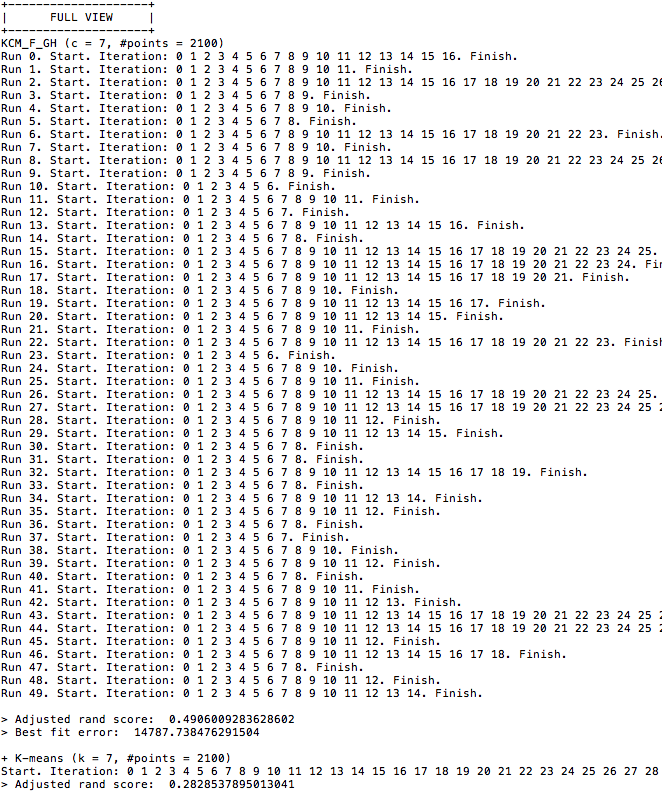
\includegraphics[width=0.50\textwidth]{part_i_full.png}
\caption{Output log of Part I on full view (RGB + shape). We run KCM-F-GH $num\_times = 50$ with random initial representatives in each cluster. Then, we pick the best fitting KCM-F-GH and compute its adjusted rand index (see bottom). KCM-F-GH achieved $ari_\textit{KCM-F-GH} = 0.4906$ while $k$-means achieved $ari_\textit{k-means} = 0.2826$.}
\end{figure}

\begin{figure}
\label{part_i_rgb}
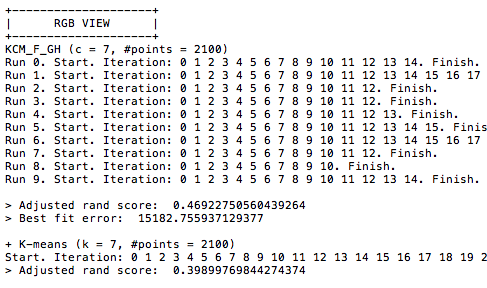
\includegraphics[width=0.50\textwidth]{part_i_rgb.png}
\caption{Output log of Part I on full view (RGB). We run KCM-F-GH $num\_times = 10$ with random initial representatives in each cluster. Then, we pick the best fitting KCM-F-GH and compute its adjusted rand index (see bottom). KCM-F-GH achieved $ari_\textit{KCM-F-GH} = 0.4692$ while $k$-means achieved $ari_\textit{k-means} = 0.3990$.}
\end{figure}

\section{Part II - Supervised Learning}

\subsection{Implementation}

The test code start point is located in \textit{part\_2.py}.
In the first moment, we perform a grid search in the training dataset to find the best hyper-parameters for the classifiers.
Then, we run cross-validation multiple times in the training dataset to estimate the accuracy (and its standard deviation) for each classifier.
After that, we run the classifiers on the test dataset to evaluate the overall accuracy.
Last, we perform the Friedman test to compare all pairs of classifiers.
The program writes the output log into \textit{part\_2\_log.txt}.

Each classifier contains two main methods: \textit{fit} and \textit{predict}.
\begin{itemize}
\item \textit{gaussian\_mle.py}: defines class \textit{GaussianMLE}.
In its method \textit{fit}, the training dataset is split up into subsets sharing the same label.
Then, the gaussian distribution parameters (\textit{i.e.}, the mean $\mu$ and the covariance matrix $\Sigma$) are estimated for each class.
Once trained, the MLE classifier is also able to compute the a posteriori probabilities for a given point.
This is needed for the hybrid classifier.
\item \textit{knn\_classifier.py}: defines class \textit{KNNClassifier}.
It performs no computation in the method \textit{fit}.
Instead, it only stores the labeled points.
In the method \textit{predict}, we then compute the distances from each input point to all examples and use a heap to keep track of the nearest $k$ points.
The predicted label is computed by picking the class of the majority.
\item \textit{combinex\_max\_classifier.py}: defines class \textit{CombinedMaxClassifier}, the hybrid classifier.
It takes a list of views to be tested on the dataset, and the hyper-parameter $k$ for its KNN classifiers.
Internally, it performs a cartesian product between the list of classifiers (MLE and KNN) and all views.
It forwards \textit{fit} and \textit{predict} to all its classifier-view pairs, and returns the combined answer.

\end{itemize}

\subsection{Experiments and Results}

\begin{figure}
\label{part_ii_results}
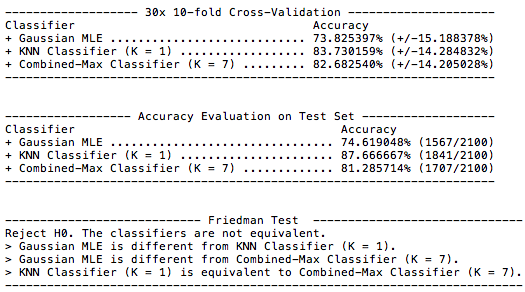
\includegraphics[width=0.50\textwidth]{part_ii_results.png}
\caption{Output log of Part II. The first section shows the average accuracy and its error margin measured by running 10-fold cross-validation 30 times on the training dataset. The second section shows the overall accuracy measured on the test dataset. The last section shows the Friedman test result (on the training dataset).}
\end{figure}

Grid-search finds that the optimal hyper-parameters are $k = 1$ for KNN and $k = 7$ for the hybrid method.
Figure \ref{part_ii_results} was taken from the output log of Part II.
As we can see in the cross-validation table, Gaussian MLE has the lowest average accuracy among all classifiers ($\approx74\%$), while both hybrid and KNN achieve similarly higher accuracies ($\approx 83\%$).
On the complete test set containing $2100$ points, KNN achieves the highest accuracy, followed by hybrid and then Gaussian MLE.
In fact according to the Friedman test results, KNN and hyrid are statistically equivalent.

When it comes to the comparative computational costs, KNN is certainly cheaper than hybrid, since hybrid needs to run multiple classifiers internally before combining their answers.
Gaussian MLE is indeed the cheapest method, because its prediction consists only of simple likelihood computations.

\section{Conclusion}

\textbf{Part I}. KCM-F-GH outperforms the standard $k$-means, but it is dozens of times slower than it.
It may be achieve better results in different datasets.
However, on the segmentation dataset it has more drawbacks than advantages.
Perhaps, the instrinsic nature of this data does not fit well with gaussian kernels (and therefore, its related algorithms).

\textbf{Part II}. KNN achieved the best tradeoff between accuracy and computational cost.
Though Gaussian MLE is linear in complexity, it tends to be less accurate than KNN (on this particular dataset).
Furthermore, additional optimizations in KNN, like the usage of spatial datastructures to store points, may improve considerably its performance on large datasets.
Another advantage is its hyper-parameter $k$, which makes it more robust to noise in data.

\begin{thebibliography}{00}
\bibitem{b1} Francisco de A.T. de Carvalho, Eduardo C. Simões, Lucas V.C. Santana, Marcelo R.P. Ferreira,
Gaussian kernel c-means hard clustering algorithms with automated computation of the width hyper-parameters,
Pattern Recognition,
Volume 79,
2018,
Pages 370-386,
ISSN 0031-3203,
https://doi.org/10.1016/j.patcog.2018.02.018.

\bibitem{b2} Vision Group, University of Massachusetts, 
Image Segmentation Data,
http://archive.ics.uci.edu/ml/machine-learning-databases/image/.

\end{thebibliography}

\end{document}
